\documentclass[twoside]{article}

\usepackage{amsmath,amsthm,amssymb,graphicx}
\usepackage{hyperref}
\usepackage[numbers]{natbib}
\usepackage{float}

\theoremstyle{definition}
\newtheorem{thm}{Theorem}[section]
\newtheorem{lem}[thm]{Lemma}
\newtheorem{prop}[thm]{Proposition}
\newtheorem{cor}[thm]{Corollary}
\newenvironment{pf}{{\noindent\sc Proof. }}{\qed}
\newenvironment{map}{\[\begin{array}{cccc}} {\end{array}\]}

\newcommand{\comment}[1]{}
\theoremstyle{definition}
\newtheorem*{defn}{Definition}
\newtheorem*{exmp}{Example}
\newtheorem*{prob}{Problem}

\theoremstyle{remark}
\newtheorem*{rem}{Remark}
\newtheorem*{note}{Note}
\newtheorem*{exer}{Exercise}

\setlength{\oddsidemargin}{0.25 in}
\setlength{\evensidemargin}{-0.25 in}
\setlength{\topmargin}{-0.6 in}
\setlength{\textwidth}{6.5 in}
\setlength{\textheight}{8.5 in}
\setlength{\headsep}{0.75 in}
\setlength{\parindent}{0 in}
\setlength{\parskip}{0.1 in}

\newcommand{\widgraph}[2]{\includegraphics[keepaspectratio,width=#1]{#2}}
\newcommand{\widgraphr}[3]{\includegraphics[keepaspectratio,width=#1,angle=#3]{#2}}

\newcommand{\lecture}[4]{
   \pagestyle{myheadings}
   \thispagestyle{plain}
   \newpage
   \setcounter{page}{1}
   \noindent
   \begin{center}
   \framebox{
      \vbox{\vspace{2mm}
    \hbox to 6.28in { {\bf Stat365/665 (Spring 2015) Data Mining and Machine Learning \hfill Lecture: #4} }
       \vspace{6mm}
       \hbox to 6.28in { {\Large \hfill #1  \hfill} }
       \vspace{6mm}
       \hbox to 6.28in { {\it Lecturer: #2 \hfill Scribe: #3} }
      \vspace{2mm}}
   }
   \end{center}
   \markboth{#1}{#1}
   \vspace*{4mm}
}


%%%%%%%
% Some commonly used notation
%%%%%%%

\def\R{{\mathbb R}}
\def\X{{\mathcal X}}
\def\Y{{\mathcal Y}}
\def\H{{\mathcal H}}
\def\E{{\mathbb E}}
\def\sign{{\rm sign}}

\newcommand{\percent}{$\%$}

\begin{document}

\lecture{STATS 665 Homework 2}{Leon Lixing Yu}{Leon Lixing Yu}{1}

\section{Problem 1}
\subsection{closed form of $\hat \beta$}
$\hat \beta$ is given by:\[ \hat \beta = \underset{\beta}{\operatorname{argmin}}  \frac{1}{2}\|X\beta - y\|_2^2 + \lambda\|\beta\|_2^2\] 
In order to find $argmin$, we need to take the derivative of the loss function and make it equal to 0. In this assignment, I will use
the notation, $x_j^{(i)}$, to denote that for the given data ${(x^{(i)},y^{(i)})}_{i=1}^n$, $x_j^{(i)}$ is the $j$th element of $x^{(i)}$, where $x^{(i)} \in \R^d, y \in \R$, $X \in \R^{d\times n}, Y \in \R^n$. 
Therefore, we have:
\[ \frac{d}{d\beta_j}l(\beta | X,Y) = (\overset{n}{\underset{i=1}{{\Sigma}}}((\overset{d}{\underset{j=1}{{\Sigma}}}x_j^{(i)}\beta_j) - y^{(i)})^2 + \lambda\overset{d}{\underset{j=1}{{\Sigma}}}\beta_j^2)^\prime = 0\]
\[ \Rightarrow 2X^T(X\beta - Y) + 2\lambda\textbf(I_d)\beta = 0\]
\[ \Rightarrow \hat \beta = (X^TX + \lambda\textbf(I_d))^{-1}X^TY\]

\subsection{Find a simple expression for $\| \hat \beta - \beta^* \|$}
FIXME
\subsection{Find a closed form of $\hat f$}
Notation Note: Following the previous convention, I am using ${(x^{(i)},y^{(i)})}_{i=1}^n$ instead of ${(x_i,y_i)}_{i=1}^n$ to represent the dataset.
In this question, I use $f(x^{(i)})$ and $<f, \phi(x^{(i)})>$ interchangably. 
We know that:
\[ f \in \H \Rightarrow \quad f(x^{(i)}) \in \H \Rightarrow \quad <f, \phi(x^{(i)})> \in \H\]
With the notation given, we have equation:
\[ \hat f = \underset{f}{\operatorname{argmin}} \sum_{i=1}^n (y^{(i)} -  <f, \phi(x^{(i)})>_\H)^2 + \lambda \|f\|_\H^2\]
Using representer theorm, we have:
\[ f = \sum_{i=1}^n\alpha^{(i)}\phi(x^{(i)})= \sum_{i=1}^n\alpha^{(i)}k(x^{(i)},\cdot)\]
The equation above means $f$ is a linear combination of feature space, mapping of points. substitute the relation above into the original $\hat f$ equation, we have:
\[ \sum_{i=1}^n (y^{(i)} -  <f, \phi(x^{(i)})>_\H)^2 + \lambda \|f\|_\H^2=\|Y-K\boldsymbol\alpha\|^2+\lambda\boldsymbol\alpha^TK\boldsymbol\alpha\]
Taking derivative over $\alpha$ and make it equal to 0 to get $\underset{\alpha}{\operatorname{argmin}}$:
\[\frac{d}{d\alpha}(\|Y-K\boldsymbol\alpha\|^2+\lambda\boldsymbol\alpha^TK\boldsymbol\alpha) = 0\]
\[\Rightarrow 2K(Y - K\boldsymbol\alpha)+2\lambda\mathbf{I_d}K\boldsymbol\alpha = 0\]
\[\Rightarrow (K+ \lambda\mathbf{I_d})\boldsymbol\alpha = 2Y\]
\[\Rightarrow \boldsymbol{\hat \alpha} = (K +  \lambda\mathbf{I_d})^{-1}Y\]

recall:
\[ f = \sum_{i=1}^n\alpha^{(i)}\phi(x^{(i)})= \sum_{i=1}^n\alpha^{(i)}k(x^{(i)},\cdot)\]
our $\hat f$ is then:
\[\hat f = K^T\boldsymbol{\hat \alpha}= K^T (K +  \lambda\mathbf{I_d})^{-1}Y\] In which $K$ is the Kernel matrix W.R.T $X$
\subsection{implement the solution of $\hat f$ in matlab}
The code for this part is attached in \textbf{Appendix A: problem 1 Code}, I use Gaussian Kernel because it is the first one I tried and it worked pretty well. I have attached a few graphs to show the differences between real label value and decision values got from $\hat f$.\\
To have a perfect fit, I adujust the values of $\lambda$ and $\sigma$. 
Multiple attempts are shown below with descriptions.
\begin{figure}[H]
\centering
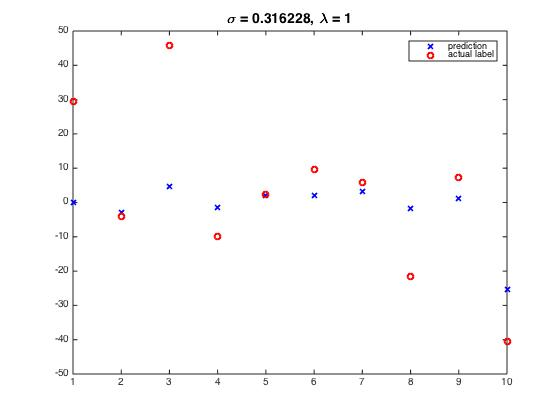
\includegraphics[width=120mm]{problem1Pic1.jpg}
\caption{Red circle indicates labels, blue cross is the $\hat f$ value. $n=10, \lambda =1, \sigma^2 = 0.1$ in this test case. I see that when $x^{(i)}$ is close to decision boundary, 0, it is more accurate in this setting.It is an underfit case.  \label{problem1Pic1}}
\end{figure}

\begin{figure}[H]
\centering
\includegraphics[width=120mm]{problem1Pic2.jpg}
\caption{ $\lambda =1, \sigma = 1$ in this test case. I see that most of the $x^{(i)}$ can be predicted accurately with two exceptions at the end of the decision boundary   \label{problem1Pic2}}
\end{figure}

\begin{figure}[H]
\centering
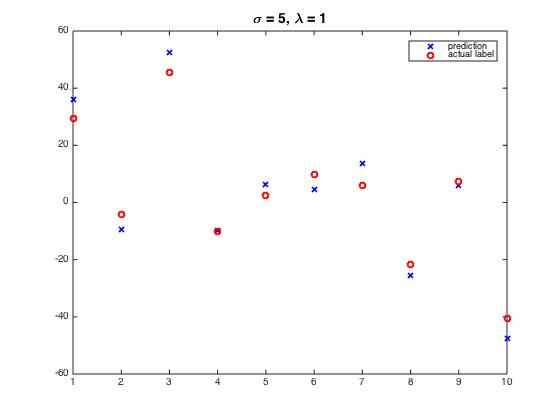
\includegraphics[width=120mm]{problem1Pic3.jpg}
\caption{ $\lambda =1, \sigma = 5$ in this test case. Though the $x^{(i)}$ at both ends are better predicted, the average accuracy has dropped.    \label{problem1Pic2}}
\end{figure}

\begin{figure}[H]
\centering
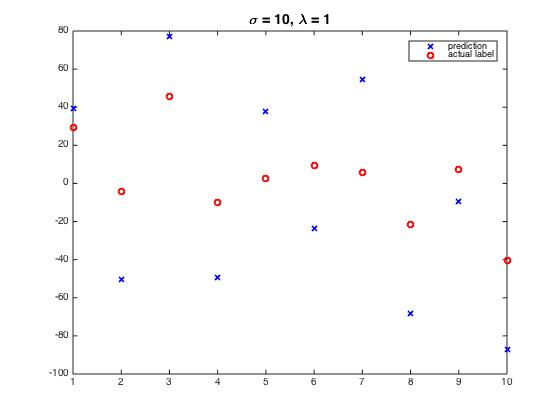
\includegraphics[width=120mm]{problem1Pic4.jpg}
\caption{ $\lambda =1, \sigma = 10$.  All $x^{(i)}$ are fitted badly. It is clearly a case of over fitting.  \label{problem1Pic2}}
\end{figure}

\begin{figure}[H]
\centering
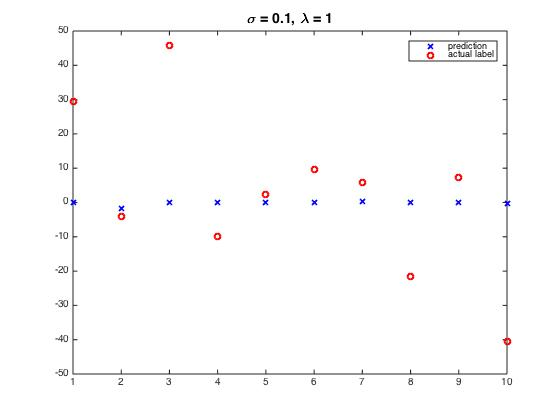
\includegraphics[width=120mm]{problem1Pic5.jpg}
\caption{ $\lambda =1, \sigma = 0.1$.  It is clearly a case of under fit. It is way under fit so that the decision boundary looks like a straight line.  \label{problem1Pic2}}
\end{figure}

\begin{figure}[H]
\centering
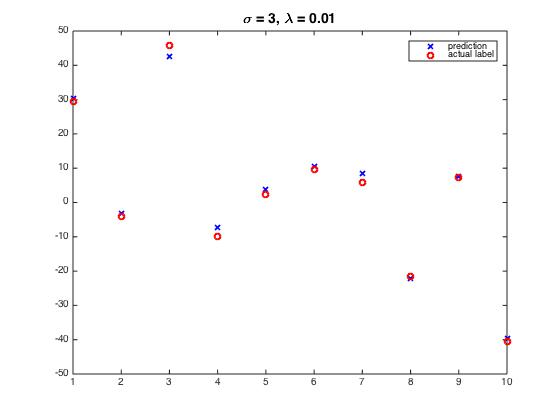
\includegraphics[width=120mm]{problem1Pic6.jpg}
\caption{ $\lambda =0.01, \sigma = 3$.  Most of the predictions for $x^{(i)}$ tends to overlap with their labels or be really close to their actual labels. I consider this is a good fit for the test data. \label{problem1Pic2}}
\end{figure}

\section{Problem 2}
\subsection{Heatmap of learned function}
The Matlab code for this problem is attached in \textbf{Appendix B: problem 2 code}. I use $libsvm$ library for this problem. I fixed the $\sigma$ to 1. The heatmap is attached below for both training dataset and testing dataset.
  
\begin{figure}[H]
\centering
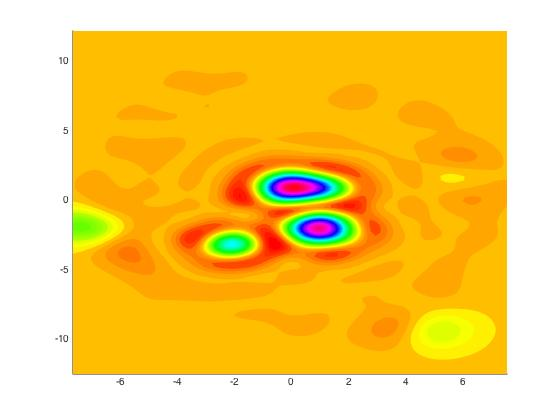
\includegraphics[width=120mm]{sigma_1_color.jpg}
\caption{ $\sigma = 1$. This heatmap is for training dataset,we can clearly see the decision boundary based on the heatmap\label{problem1Pic2}}
\end{figure}


\section{Problem 3}
\subsection{Show $k(x,y)$ is a valid kernel}
We know that kernel is a function that maps $\chi \times \chi \rightarrow \R$. 
We also know that kernel is valid if and only if for ${x_i}_{i=1}^n \in \chi, K_{ij} = k(x_i,x_j)$ is PSD. We need to prove these two statements.\\ 
Proving $k(x,y)$ maps $\chi \times \chi \rightarrow \R$:\\ 
Assuming:
\[k_1(x,y) = <\Phi_1(x),\Phi_1(y)>\]
\[k_2(x,y) = <\Phi_2(x),\Phi_2(y)>\]
Since $k_1(x,y)$ and $k_2(x,y)$ are vaild kernel, they both maps $\chi \times \chi \rightarrow \R$. 
we now have 
\[k(x,y) = <\Phi_1(x),\Phi_1(y)>\cdot <\Phi_2(x),\Phi_2(y)>\]
\[\Rightarrow k(x,y) = (\Phi_1(x)^T \Phi_1(y))\cdot(\Phi_2(x)^T\Phi_2(y))\]
\[\Rightarrow k(x,y) \in \R\]
We also know that $(x,y) \in \R^\chi$, so $k(x,y)$ maps $\chi \times \chi \rightarrow \R$.\\
Proving $k(x,y)$ is PSD:
\[K_{ij} = k(x_i,x_j) =  <\Phi(x_i),\Phi(x_j)> =\Phi(x_i)^T\Phi(x_j) \]
\[\upsilon^T K \upsilon = \sum_i^n \sum_j^n \upsilon_i K_{ij} \upsilon_j\]
\[=\sum_i^n \sum_j^n \upsilon_i \Phi(x_i)^T\Phi(x_j) \upsilon_j\]
\[=\sum_i^n \sum_j^n \upsilon_i \sum_l^n \phi_l(x_i)^T\phi_l(x_j) \upsilon_j\]
\[=\sum_l^n \sum_i^n \sum_j^n \upsilon_i \phi_l(x_i)^T\phi_l(x_j) \upsilon_j\]
\[=\sum_l^n(\sum_i^n \upsilon_i \phi_l(x_i))^2 \geq 0\]



 
end of the story

\end{document}
